\section{Inequalities and identities}
\label{sec:appendix_identities}

\subsection{Jensen's inequality}
\begin{prop}
(Jensen's inequality) 
If $f(x)$ is a convex function, then for any distribution $p(x)$,
$$ \mathbb{E}_{p(x)}[f(x)] \geq f(\mathbb{E}_{p(x)}[x]) .$$
\end{prop}
%
A visual proof is provided in Figure \ref{fig:appendix_jensen}.

\begin{figure}[ht]
 \centering
 \subfigure[for discrete distributions]{
 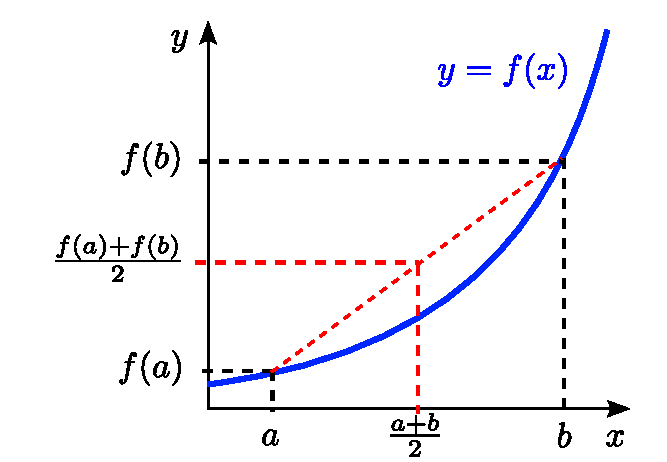
\includegraphics[width=0.45\linewidth]{Appendix1/jensen_discrete.pdf}}
 \hfill
 \subfigure[for continuous distributions]{
 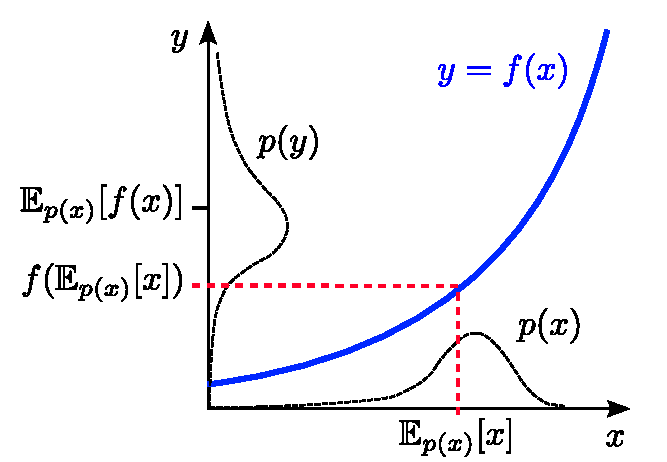
\includegraphics[width=0.45\linewidth]{Appendix1/jensen.pdf}}
 \caption{A visual proof of the Jensen's inequality. }
 \label{fig:appendix_jensen}
\end{figure}


\subsection{H{\"o}lder's inequality}
\begin{prop}
(H{\"o}lder's Inequality)
Let $(\mathcal{X}, \Sigma, \mu)$ be a measure space and let $p, q \in [1, +\infty]$ satisfying $\frac{1}{p} + \frac{1}{q} = 1$, then for all measurable functions $f$, $g$ on $\mathcal{X}$,
$$ \int | f(x) g(x) | d \mu \leq \left( \int | f(x) |^p d \mu \right)^{\frac{1}{p}} \left( \int | g(x) |^q d \mu \right)^{\frac{1}{q}} .$$
\end{prop}
Setting $p = q = 2$ recovers the Cauchy-Schwarz inequality.
%
\begin{proof}
We assume $\exists x \in \mathcal{X} \text{ s.t. } f(x) \neq 0$ w.l.o.g., then
\begin{equation*}
\begin{aligned}
 \int | f(x) g(x) | d \mu &= \left( \int | f(x) |^p d \mu \right) \int [ ( | g(x) | | f(x) |^{1 - p} )^{q} ]^{\frac{1}{q}} \frac{|f(x)|^p}{ \int | f(x) |^p d \mu } d \mu \\
 &\leq \left( \int | f(x) |^p d \mu \right) \left[ \int ( | g(x) | | f(x) |^{1 - p} )^{q} \frac{|f(x)|^p}{ \int | f(x) |^p d \mu } d \mu \right]^{\frac{1}{q}} \\
 &= \left( \int | f(x) |^p d \mu \right)^{1 - \frac{1}{q}} \left[ \int | g(x) |^{q} d \mu \right]^{\frac{1}{q}} \\
 &= \left( \int | f(x) |^p d \mu \right)^{\frac{1}{p}} \left[ \int | g(x) |^{q} d \mu \right]^{\frac{1}{q}}.
\end{aligned}
\end{equation*}
For the second line we used the Jensen's inequality, with the function $h(x) = x^{\frac{1}{q}}$ which is convex when $q >= 1$, and the probability measure $p(x) = \frac{|f(x)|^p}{ \int | f(x) |^p d \mu }$. For the third and the last lines we used the assumption that $\frac{1}{p} + \frac{1}{q} = 1$.
\end{proof}

\subsection{Stein's identity}
We provide a proof of Stein's identity in 1D case. The general case can be proved accordingly.
\begin{prop}
(Stein's identity, one dimensional case)
Let $p(x)$ be a differentiable probability density function of $x \in \mathbb{R}$. Let $h(x)$ be a function such that $\lim_{x \rightarrow \pm \infty} p(x) h(x) = 0$. Then
$$\mathbb{E}_{p}[h(x) \nabla_{x} \log p(x) + \nabla_{x} h(x) ] = 0 .$$ 
\end{prop}

\begin{proof}
Using integration by parts, we have
\begin{equation*}
\begin{aligned}
\mathbb{E}_{p}[h(x) \nabla_{x} \log p(x) + \nabla_{x} h(x) ] &= \int p(x) h(x) \nabla_{x} \log p(x) dx + \int p(x) \nabla_{x} h(x) dx \\
&= \int h(x) \nabla_{x} p(x) dx + \int p(x) \nabla_{x} h(x) dx \\
&= \int \nabla_{x} [h(x) p(x)] dx \\
&= h(x) p(x) |_{-\infty}^{+\infty} = 0. \quad\quad \text{// boundary condition}
\end{aligned}
\end{equation*}
\end{proof}

\cite{stein:stein_method1972} proposed the following lemma for Gaussian distribution.
\begin{lemma}
(\citep{stein:stein_method1972})
Let $p(x) = \mathcal{N}(x; \mu, \sigma^2)$, and the function $h(x)$ satisfies $| \mathbb{E}_{p}[g(x) (x - \mu)] |< +\infty$ and $|\mathbb{E}_{p}[\nabla_{x} g(x)] | < +\infty$. Then
$$ \mathbb{E}_{p}[g(x) (x - \mu)] = \sigma^2 \mathbb{E}_p[\nabla_{x} g(x)]. $$
\end{lemma}

Later, \cite{chen:poisson1975} extended the characterisation to Poisson distribution.
\begin{lemma}
(\citep{chen:poisson1975}) A random variable $x$ taking values in $\mathbb{N}$ is Poisson distributed with rate $\lambda$, if and only if $P(x)$ satisfies
$$ \mathbb{E}_{P}[ \lambda h(x+1) - xh(x) ] = 0 $$
for all bounded functions $h: \mathbb{N} \rightarrow \mathbb{R}$.
\end{lemma}
\begin{proof}
Assume $x$ is Poisson distributed with rate $\lambda$, then
\begin{equation*}
\begin{aligned}
\mathbb{E}_{P}[ \lambda h(x+1) - xh(x) ] 
& = \sum_{n=0}^{+\infty} \lambda h(n+1) \exp[-\lambda] \frac{\lambda^n}{n!} - \sum_{n=0}^{+\infty} n h(n) \exp[-\lambda] \frac{\lambda^n}{n!} \\
& = \sum_{n=1}^{+\infty} h(n) \exp[-\lambda] \frac{\lambda^n}{(n-1)!} - \sum_{n=1}^{+\infty} h(n) \exp[-\lambda] \frac{\lambda^n}{(n - 1)!} = 0. \\
\end{aligned}
\end{equation*}
Conversely if the identity holds for every function $h(x)$, then setting $h(x) = \delta_{x - k}$ for some $k$, by assumption we have
$$ \mathbb{E}_{P}[ \lambda h(x+1) - xh(x) ] = \lambda P(x = k - 1) - k P(k) = 0,$$
which implies 
$$ \frac{P(x = k)}{P(x = k-1)} = \frac{\lambda}{k} = \frac{\text{Poisson}_{\lambda}( x = k)}{ \text{Poisson}_{\lambda}( x = k - 1) }.$$
Since it holds for all $k \in \mathbb{N}^{+}$, we conclude that $x$ is Poisson distributed.
\end{proof}
